% How a training pair (theta, x) is built: nuisances at the simulation stage are baked into the stored
% seismograms; nuisances at the training stage are drawn afresh every time the dataloader serves them.
% Compile:  pdflatex nuisance_stages.tex ; pdftoppm -png -r 200 nuisance_stages.pdf nuisance_stages
\documentclass[tikz,border=10pt]{standalone}
\usepackage{amsmath}
\usepackage{newtxtext,newtxmath}
\usetikzlibrary{arrows.meta,positioning,fit,backgrounds,calc}

\begin{document}
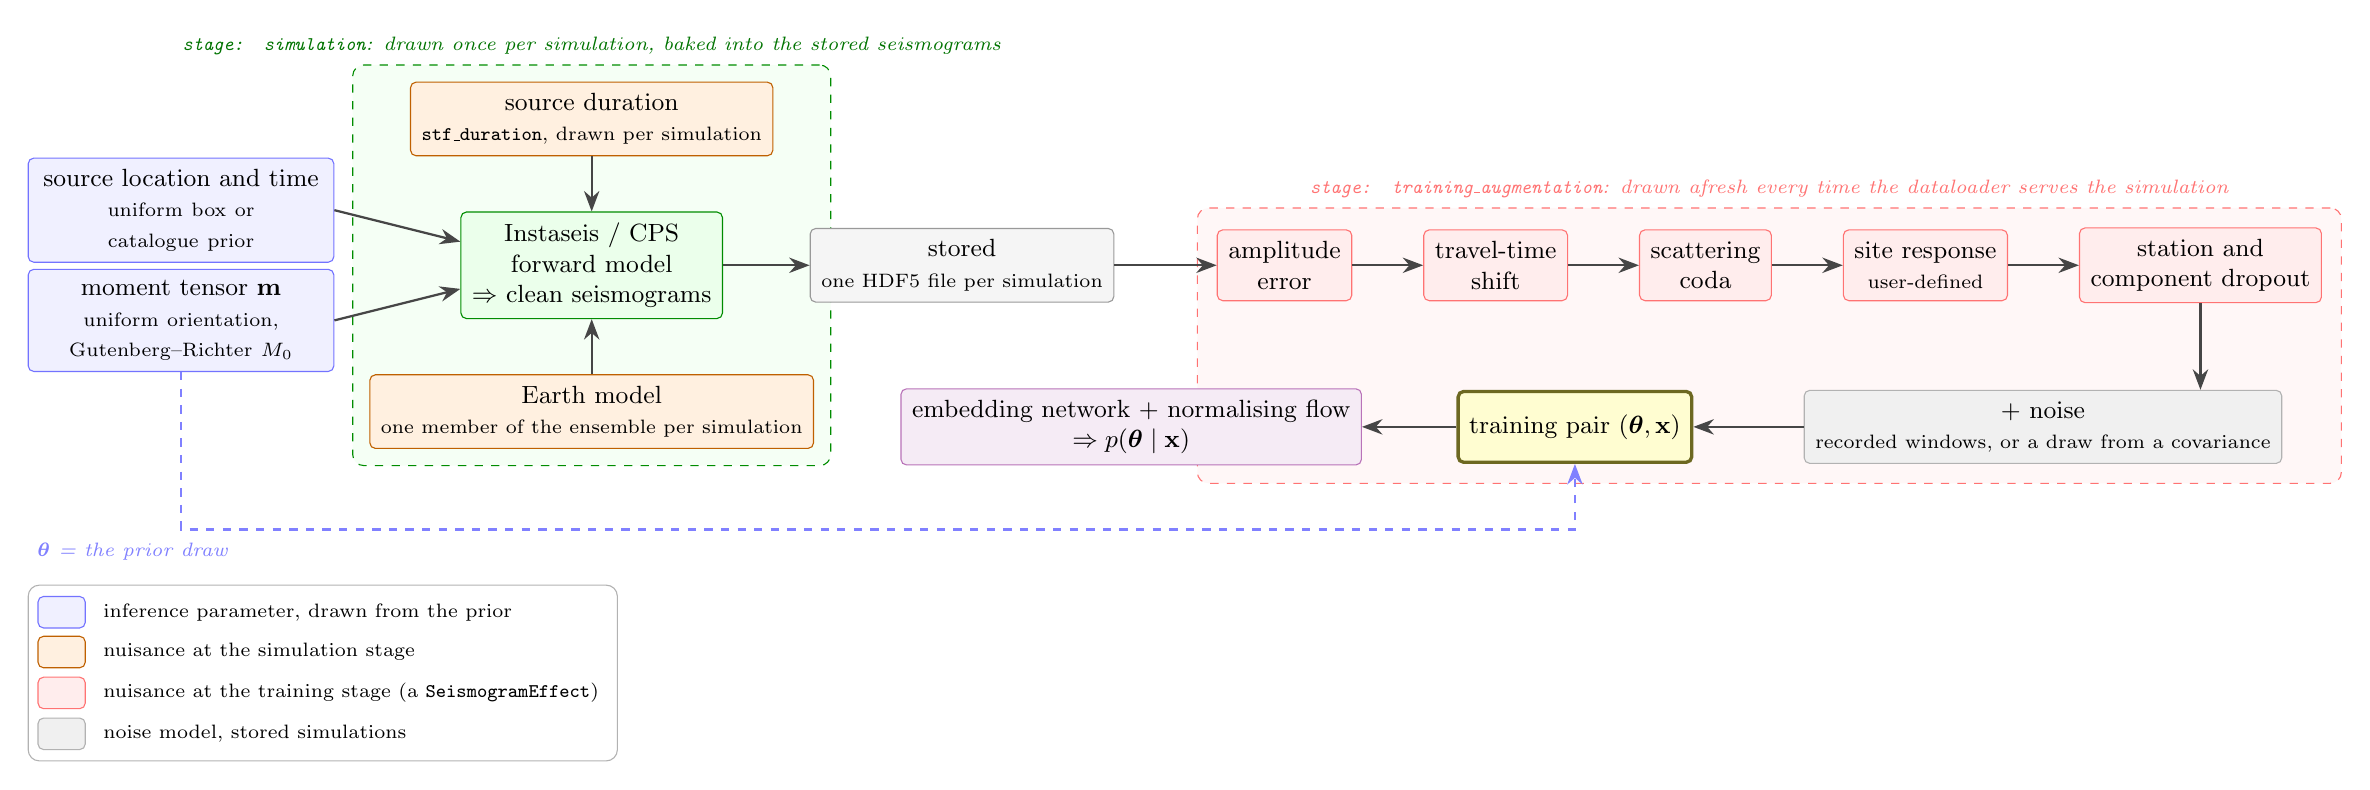
\begin{tikzpicture}[
  font=\small,
  >={Stealth[length=2.6mm]},
  node distance=6mm and 9mm,
  box/.style={draw, rounded corners=2pt, align=center, inner sep=4pt, minimum height=9mm, fill=white},
  prior/.style={box, fill=blue!6, draw=blue!55, text width=36mm},
  sim/.style={box, fill=green!8, draw=green!55!black},
  simn/.style={box, fill=orange!12, draw=orange!75!black},
  aug/.style={box, fill=red!7, draw=red!55},
  noise/.style={box, fill=gray!12, draw=gray!60},
  outbox/.style={box, fill=yellow!18, draw=olive!70!black, very thick},
  flow/.style={->, thick, gray!55!black},
  lbl/.style={font=\scriptsize\itshape, text=black!65},
]

% ---- forward model with its two prior inputs -----------------------------
\node[sim] (gf) {Instaseis / CPS\\forward model\\$\Rightarrow$ clean seismograms};
\node[prior, left=16mm of gf, yshift=7mm]  (loc) {source location and time\\\scriptsize uniform box or catalogue prior};
\node[prior, left=16mm of gf, yshift=-7mm] (mt)  {moment tensor $\mathbf{m}$\\\scriptsize uniform orientation, Gutenberg--Richter $M_0$};

% ---- simulation-stage nuisances, entering the forward model ---------------
\node[simn, above=7mm of gf] (stf) {source duration\\\scriptsize\texttt{stf\_duration}, drawn per simulation};
\node[simn, below=7mm of gf] (vel) {Earth model\\\scriptsize one member of the ensemble per simulation};

% ---- stored simulations ----------------------------------------------------
\node[noise, right=11mm of gf, draw=black!40, fill=black!4] (h5) {stored\\\scriptsize one HDF5 file per simulation};

% ---- training-stage chain ---------------------------------------------------
\node[aug, right=13mm of h5] (amp) {amplitude\\error};
\node[aug, right=of amp]   (shift) {travel-time\\shift};
\node[aug, right=of shift] (coda)  {scattering\\coda};
\node[aug, right=of coda]  (site)  {site response\\\scriptsize user-defined};
\node[aug, right=of site]  (drop)  {station and\\component dropout};
\node[noise, below=11mm of drop, xshift=-20mm] (noise) {$+$ noise\\\scriptsize recorded windows, or a draw from a covariance};

% ---- output ----------------------------------------------------------------
\node[outbox, left=14mm of noise] (pair) {training pair $(\boldsymbol\theta, \mathbf{x})$};
\node[box, left=12mm of pair, fill=violet!8, draw=violet!55] (npe) {embedding network $+$ normalising flow\\$\Rightarrow p(\boldsymbol\theta \mid \mathbf{x})$};

% ---- arrows ------------------------------------------------------------------
\draw[flow] (loc.east) -- ($(gf.west)+(0,3mm)$);
\draw[flow] (mt.east)  -- ($(gf.west)-(0,3mm)$);
\draw[flow] (stf) -- (gf);
\draw[flow] (vel) -- (gf);
\draw[flow] (gf) -- (h5);
\draw[flow] (h5) -- (amp);
\draw[flow] (amp) -- (shift);
\draw[flow] (shift) -- (coda);
\draw[flow] (coda) -- (site);
\draw[flow] (site) -- (drop);
\draw[flow] (drop.south) -- (drop.south |- noise.north);
\draw[flow] (noise) -- (pair);
\draw[flow] (pair) -- (npe);
% theta: the prior draw is the label of the training pair
\draw[flow, dashed, blue!50] (mt.south) -- ++(0,-20mm) -| (pair.south);
\node[lbl, text=blue!50, anchor=north west] at ($(mt.south west)+(0,-20.5mm)$) {$\boldsymbol\theta$ = the prior draw};

% ---- stage backgrounds ---------------------------------------------------------
\begin{scope}[on background layer]
  \node[draw=green!55!black, dashed, rounded corners, fill=green!4, fit=(stf)(gf)(vel), inner sep=6pt,
        label={[lbl,text=green!45!black]above:{\texttt{stage: simulation}: drawn once per simulation, baked into the stored seismograms}}] {};
  \node[draw=red!55, dashed, rounded corners, fill=red!3, fit=(amp)(drop)(noise), inner sep=7pt,
        label={[lbl,text=red!55]above:{\texttt{stage: training\_augmentation}: drawn afresh every time the dataloader serves the simulation}}] {};
\end{scope}

% ---- legend -------------------------------------------------------------------
\matrix[draw=black!30, rounded corners, anchor=north west, nodes={anchor=west, font=\scriptsize},
        row sep=1.5pt, column sep=3pt] (leg) at ($(mt.south west)+(0,-27mm)$) {
  \node[prior, text width=, minimum height=4mm, minimum width=6mm]{}; & \node{inference parameter, drawn from the prior}; \\
  \node[simn, minimum height=4mm, minimum width=6mm]{};  & \node{nuisance at the simulation stage}; \\
  \node[aug, minimum height=4mm, minimum width=6mm]{};   & \node{nuisance at the training stage (a \texttt{SeismogramEffect})}; \\
  \node[noise, minimum height=4mm, minimum width=6mm]{}; & \node{noise model, stored simulations}; \\
};

\end{tikzpicture}
\end{document}
